\chapter{Flux-limited Diffusion for Multiple Scattering in Participating Media}
\label{sec:fld}

We have seen in the previous chapter, that the first order truncation of the $P_N$-equations can be collapsed into a simple diffusion equation, which has a low memory footprint and can be solved very efficiently using a Multigrid solver. The diffusion approximation therefore offers significant advantages over the $P_N$-method in terms of required computational resources. At the same time, it gives only a poor approximation to the ground truth result, due to the very coarse angular discretization.

In this chapter, flux-limited diffusion is introduced to the problem of rendering participating media in computer graphics. The theory has been invented in the astrophysics domain and is primarily attributed to Levermore et al.~\cite{Levermore81}. Their work introduces the theory and discusses its properties for certain canonical problems, such as a single point source within a homogeneous participating medium. In this chapter, a novel numerical method is deviced, based on flux-limited diffusion theory. It allows to solve for the fluence on a finite difference grid with higher accuracy comppred to the diffusion approximation, at a significantly lower cost. The results have been published in~\cite{Koerner14}.

This chapter continues with revisiting the moment problem from section~\ref{sec:moment_closure} and introduces the flux-limit constraint, which is violated by diffusion and causes energy loss. The streaming transport regime is introduced, for which an advection equation is derived in section~\ref{sec:fld_streaming_limit_approximation}. Flux-limited diffusion is derived as a means to blend between the two extreme modes of transport using local information. This blending is driven by the variable Eddington factor, which is introduced in section~\ref{sec:fld_vef}. Various concrete realizations of the eddington factor are given and compared in section~\ref{sec:fld_vef_factors}. Finally, an iterative solver is presented in section~\ref{sec:fld_solver}. The chapter concludes with results in section~\ref{sec:fld_results}.


\section{Moment Problem Revisited}
\label{sec:moment_problem_revisited}

In section~\ref{sec:moment_closure}, it was established that a choice for the second moment of the radiance distribution was required to close the system of equations, which was found by collapsing the moment expansion of the radiative transfer equation, truncated after the first moment. The classical diffusion approximation was derived by assuming an isotropic radiance distribution for the second moment. In this section, we will take a closer look at the moments and carve out an important feature, which explains the bad accuracy of classical diffusion approximation in certain scenarios.

The distribution of power $\phi$ over solid angle was given by the normalized radiance $\widehat{L}$. Since it is a probability distribution, it has to integrate to one, which is easily verified
\begin{align*}
\int_{\Omega}{\hat{L}(\vec{x}, \omega)\ud\omega}=
\int_{\Omega}{\frac{L\left(\vec{x}, \omega\right)}{\phi\left(\vec{x}\right)}\ud\omega}=
\frac{1}{\phi\left(\vec{x}\right)}
\int_{\Omega}{L\left(\vec{x}, \omega\right)\ud\omega}
=1
=\hat{L}_0
\end{align*}
Further, we have that the normalized radiance $\widehat{L}$ has to be non-negative, in order to be a probability distribution:
\begin{align*}
\hat{L}(\vec{x}, \omega)\ge 0 \qquad \text{for all unit directions } \omega
\end{align*}
which is easily verified from the fact, that the radiance field is non-negative by definition:
\begin{align*}
L\left(\vec{x}, \omega\right) \ge 0
\implies
\int_{\Omega}{L(\vec{x}, \omega)\ud\omega}=\phi\left(\vec{x}\right)\ge 0
\implies
\frac{L\left(\vec{x}, \omega\right)}{\phi\left(\vec{x}\right)}=\widehat{L}(\vec{x}, \omega) \ge 0
\end{align*}

Akhiezer~\cite{Akhiezer65} established, that the probability distribution contraints on a function results in a set of inequalities between moments of this function. In particular, the non-negativity constraint on the radiance field $L$ and its normalized distribution impose a constraint between the zero moment and the first moment. In case of the radiance field, this constraint can be derived by considering the dot product between direction vectors $\omega'$ and $\omega$, both of unit length. We have
\begin{align*}
-1 \le \omega'\cdot\omega \le 1
\implies
0 \le 1 - \omega'\cdot\omega \le 1
\implies
\int_{\Omega}{\left(1-\omega'\cdot\omega\right)L\left(\vec{x}, \omega\right)\ud\omega}\ge 0
\end{align*}
which can be rearranged into
\begin{align*}
\int_{\Omega}{\left(1-\omega'\cdot\omega\right)L\left(\vec{x}, \omega\right)\ud\omega} &\ge 0
\\
\int_{\Omega}{L\left(\vec{x}, \omega\right)\ud\omega}
-\int_{\Omega}{\omega'\cdot\omega L\left(\vec{x}, \omega\right)\ud\omega}
&\ge 0
\\
\int_{\Omega}{L\left(\vec{x}, \omega\right)\ud\omega}
-\omega'\cdot\int_{\Omega}{L\left(\vec{x}, \omega\right)\omega\ud\omega}
&\ge 0
\\
\phi\left(\vec{x}\right)
-\norm{\vec{E}\left(\vec{x}\right)}
&\ge 0
\\
\phi\left(\vec{x}\right)
&\ge \norm{\vec{E}\left(\vec{x}\right)}
\end{align*}
This constraint states, that the total power at position $\vec{x}$ must never exceed the length of the flux-vector.
\TD{intuition behind flux-limit}

A very similar constraint can be derived for the normalized radiance $\widehat{L}$, by following the same steps above. This results in
\begin{align}
\label{eq:fld_flux_limit}
1
\ge
\norm{
\frac{\vec{E}\left(\vec{x}\right)}{\phi\left(\vec{x}\right)}
}
\end{align}
In the case of the classical diffusion approximation, we have $\vec{E}\approx-D\nabla\phi$ (equation~\ref{eq:diffusion_ficks_law}). Inserting this into equation~\ref{eq:fld_flux_limit} gives
\begin{align}
\label{eq:fld_flux_limit}
1
\ge
\norm{
\frac{\nabla\phi\left(\vec{x}\right)}{3\sigma_t\left(\vec{x}\right)\phi\left(\vec{x}\right)}
}
\end{align}
Here it can be seen clearly, that with the classical diffusion approximation, this constraint can be violated when the extinction coeffient $\sigma_t$ becomes very small, meaning in the presence of very thin medium. It breaks down completely in case of vacuum $\sigma_t=0$. The constraint can also be violated if the the fluence gradient becomes very large in relation to $\sigma_t\phi$. This happens very close to point light sources and near strong density gradients in the medium.

\todo[inline]{give intuition how the assumption of isotropic radiance distribution for the 2nd order tensor of the radiance field is violated strongly near boundaries or transitions from low to high density medium}

Violation of the constraint above means, that for the classical diffusion approximation, the flux vector is much larger than what is physically possible. Since the flux vector governs light transport, the literature often referres to classical diffusion as suffering from unphysical fluxes or unphysical light transport.


\subsubsection*{A Transport Regime Measure}

The right hand side of equation~\ref{eq:fld_flux_limit} is an important measure, which allows us to detect at every point within the domain, where and to what extend the diffusion approximation fails. And for this, only local information about the moments and extinction coefficient is needed. It is an important building block for the technique presented in this chapter, which seeks to improve the accuracy of the diffusion approximation.

The flux-limit in equation~\ref{eq:fld_flux_limit} can be factorized to make its intuition more clear:
\begin{align}
\label{eq:flux_limit_factors}
\norm{
\frac{\nabla\phi\left(\vec{x}\right)}{3\sigma_t\left(\vec{x}\right)\phi\left(\vec{x}\right)}
}
=
\frac{1}{3}
l\left(\vec{x}\right)
\frac{\norm{\nabla\phi\left(\vec{x}\right)}}{\phi\left(\vec{x}\right)}
\end{align}
It consists of two factors, of which the first is the mean free path $l$, which is the inverse of the extinction coefficient and therefore parameterizes the medium. If the mean free path is small and approaches zero, we know that photons travel only very short distances in average, before they encounter another interaction with the medium. In this case the medium is very dense. If the mean free path is large, the medium is very thin and photons travel long distances before they encounter another interaction with the medium. In case of vacuum, where no medium is present, photons travel unhindered and never interact. In this case the mean free path is infinite.
\missingfigure{transport regimes according to mean free path}
The second factor in equation~\ref{eq:flux_limit_factors} is the ratio between the length of the flux-vector (according to diffusion) and the zero moment. If the magnitude of the flux-vector is small, while the total power $\phi$ is large, we can infer that the incoming radiance is distributed equally over solid angle, which means that light is coming uniformly from all directions. If the flux-vector magnitude is large in comparison to the total power, we can infer that the energy is concentrating in certain directions. In the extreme case, when the total power is equal to the flux-vector magnitude, the light comes only from a single direction.
\missingfigure{transport regimes according to moment ratio}
The two factors in equation~\ref{eq:flux_limit_factors} parameterize the transport regime according to the medium and the distribution of incoming light over solid angle respectively. Combined, they are a local measure for the transport regime in general (as perceived by diffusion). If the medium is very dense (small mean free path) and light arrives equally distributed from all directions (small moment ratio), diffusive transport is dominating and the flux-limit is not violated. The diffusion approximation is a good approximation in these scenarios. If the medium is very thin (large mean free path) and the moment ratio approaches one, we have ballistic transport and free streaming in the case of vacuum or when the ratio is exactly one.

We ignore the $1/3$ factor in equation~\ref{eq:flux_limit_factors} and introduce $R$, a transport measure according to the diffusion approximation:
\begin{align}
R\left(\vec{x}\right)
= 
\frac{\norm{\nabla\phi\left(\vec{x}\right)}}{\sigma_t\left(\vec{x}\right)\phi\left(\vec{x}\right)}
\qquad
\qquad
\begin{array}{cc}
R\left(\vec{x}\right)\rightarrow 0 : \text{diffussive transport}\\
R\left(\vec{x}\right)\rightarrow 1 : \text{streaming transport}
\end{array}
\end{align}
In section~\ref{sec:moment_closure}, the diffusion approximation was derived by assuming isotropic distribution of radiance and therefore we see the same requirement in the fux-limit contraint, where a small moment ratio is required and implies, that light is arriving equally from all directions.

The idea of flux-limited diffusion is to avoid violation of the fux-limit and consquently prevent unphysical transport. The key idea behind flux-limited diffusion is to not only assume isotropic distribution, but also allow streaming transport and use the measure $R$, to locally realize the right mix between diffusive and streaming transport. The next important building block is therefore the question of how the diffusion equation looks like in the presence of streaming transport. This is outlined in the next section. Section~\ref{sec:fld_vef} will then develop flux-limited diffusion as a combination with classical diffusion.

\section{Streaming Limit Approximation}
\label{sec:fld_streaming_limit_approximation}

In the previous section, the transport measure $R$ was introduced, which contains the factor $\norm{\nabla\phi}/\phi$. This factor approaches one as transport becomes less diffusive and enters the streaming regime. In the case of $\norm{\nabla\phi}/\phi=1$, the length of the flux-vector matches the amount of total power. In this case, light is coming from a single direction. The radiance distribution of this configuration is given as
\begin{align}
\hat{L}\left(\omega\right)=\delta_{\Omega}\left(\omega,\vec{n}\right).
\end{align}
where $\delta_{\Omega}$ is the angular Dirac delta distribution into direction $\vec{n}$. Spatial dependency is omitted and not relevant for this discussion. The moments of this distribution are:
\begin{align}
\label{eq:zero_moment_Lhat}
\hat{L}_0\left(\omega\right)&=\int_{\Omega}{\delta_{\Omega}\left(\omega,\vec{n}\right)\ud\omega} = 1\\
\label{eq:first_moment_Lhat}
\hat{L}_1\left(\omega\right)&=\int_{\Omega}{\delta_{\Omega}\left(\omega,\vec{n}\right)\omega\ud\omega} = \vec{n}\\
\label{eq:second_moment_Lhat}
\hat{L}_2\left(\omega\right)&=\int_{\Omega}{\delta_{\Omega}\left(\omega,\vec{n}\right)\omega_i\omega_j\ud\omega} = \vec{n}_i\vec{n}_j
\end{align}
The zero moment expresses that all power given by $\phi$ comes from a single direction. The second equation shows, that the first moment of a delta distribution is identical to the vector which defines that distribution ($\vec{n}$ in our case). It shall be concluded that the length of the flux-vector equals the zero moment and its direction is $\vec{n}$ (all under the assumption of a delta radiance distribution):
\begin{align}
\label{eq:iso_delta_normE}
\vec{E} = \hat{L}_1\phi = \vec{n}\phi  &\implies \norm{\vec{E}} = \phi\\
&\implies \vec{E} \parallel \vec{n} \qquad \text{($\vec{E}$ and $\vec{n}$ are parallel)}
\end{align}
The second moment equation shows that the second moment is found by the outer product of the defining vector. Therefore, assuming a delta distribution results in the following Eddington tensor (equation~\ref{eq:eddington_tensor}):
\begin{align}
T_{ij} = \vec{n}_i\vec{n}_j
\label{eq:iso_delta_T}
\end{align}
The form of the Eddington tensor for a delta distribution of radiance in angular domain is given. In the end, this tensor is to be used to approximate the second moment of the radiance field $P$ in equation~\ref{eq:general_diffusion_equation} by $T\phi\approx P$. However, this way the direction $\vec{n}$ is introduced as another unknown. The next step in the derivation is, to reformulate $T$ and eliminate of the unknown $\vec{n}$, which is possible under certain assumptions.
%An important consideration is the fact, that the vector $\vec{n}$ is scaled to infinite length under the integral sign.
% \emph{This means our delta distribution is represented by a single vector of infinite length with direction $\vec{n}$}.

Inserting the approximation $T\phi$ into the flux-vector definition (equation~\ref{eq:me_first_resolved_E}) and assuming an isotropic emission $Q$ gives:
\begin{align*}
\vec{E}&= -\frac{1}{\sigma_t'}\operatorname{div}\left (T\phi\right )
\end{align*}
The key assumption used is that the spatial variations of $T$ can be neglected. Fundamentaly, the approach is to assume, that the radiance field $L$ can be separated into a product of two functions. One depending on angle and another function depending on position. This allows to express the divergence of the second moment as a matrix product with a gradient vector:
\begin{align}
\vec{E}&= -T\left(\frac{1}{\sigma_t'}\nabla\phi\right )
\label{eq:second_moment_iso2}
\end{align}
For the derivation the normalized flux will be addressed, which is given by scaling the flux-vector with $1/\phi$:
\begin{align}
\widehat{\vec{E}} = \frac{\vec{E}}{\phi}= -T\underbrace{\left(\frac{\nabla\phi}{\sigma_t'\phi}\right )}_{=\vec{R}}
\label{eq:second_moment_iso3}
\end{align}
Equation~\ref{eq:first_moment_Lhat} showed, that $\vec{n}$ points into the same direction as the flux-vector $\vec{E}$. This means, that the result of the transformation $T$ will be a vector, which is parallel to $\vec{n}$. Since the Eddington tensor has been constructed with $T_{ij}=\vec{n}_i\vec{n}_j$, it is known that $\vec{n}$ is the only eigenvector of $T$, with an eigenvalue greater than zero. It can be concluded that (under the assumption of negligible spatial variation of $T$) the transformation $T$ is applying a scaling operation and the dimensionless gradient $\vec{R}$ is parallel to $E$. Therefore the product of tensor $T$ is expressed with $\vec{R}$ as a scaling operation and equation~\ref{eq:second_moment_iso3} then becomes:
\begin{align}
\widehat{\vec{E}} = -\lambda\left(\frac{\nabla\phi}{\sigma_t'\phi}\right )
\label{eq:second_moment_iso4}
\end{align}
With an assumption about the spatial variation of $T$, the normalized flux-vector $\hat{L}_1$ could be expressed with respect to the zero moment $\phi$ and its spatial derivatives. What remains to be done is to find an expression for the eigenvalue $\lambda$. Then an expression for $\vec{E}$ (by using $\vec{E}=\hat{L}_1\phi$) would be found, which does not depend on itsself in anyway and therefore can be used to substitute $\vec{E}$ into the zero moment equation.

Apparently, finding $\lambda$ is easy in the case of a delta distribution of radiance. In that case it is known from equation~\ref{eq:iso_delta_normE}, that $\norm{\vec{E}}=\phi$ and therefore $\norm{\vec{E}/\phi}=1$. This requires that:
\begin{align*}
%\norm[\big]{\vec{f}}=\norm[\Bigg]
\norm{\vec{E}}
=
\norm{-\lambda\left(\frac{\nabla\phi}{\sigma_t'\phi}\right )}=1
\implies
\lambda=\frac{\sigma_t'\phi}{\norm{\nabla\phi}}
\end{align*}
Note that lambda is under the vector norm, which would make the sign of lambda ambiguous (it could be positive or negative: in both cases the length of the normalized flux-vector would be one). However, as mentioned earlier, the way $T=\vec{n}_i\vec{n}_j$ is defined allows the conclusion that $\lambda$ is the only Eigenvalue of $T$ and must be greater one. This gives the final expression for the flux-vector $\vec{E}$:
\begin{align*}
\vec{E}=\widehat{\vec{E}}\phi= -\lambda\left(\frac{\nabla\phi}{\sigma_t'\phi}\right )\phi= -\frac{\nabla\phi}{\norm{\nabla\phi}}\phi
,
\end{align*}
which states that the flux-vector is the unit vector pointing into the direction of the gradient of $\phi$ scaled by $\phi$ itself. Inserting this into the collapsed $P_1$-equation (equation~\ref{eq:general_diffusion_equation}) gives:
\begin{align}
\label{eq:iso_delta_advection_equation}
\nabla\cdot\left(\frac{\nabla\phi}{\norm{\nabla\phi}}\phi\right) &= \sigma_a\phi - Q_0
\end{align}
In case of a delta distribution of radiance in angular domain and with the assumption of negligible spatial variation of $T$, the moment equation turns into an advection equation, where the zero moment quantity $\phi$ is moved around by its normalized gradient.

This section highlights that the streaming transport is best represented by advection in case of the two term expansion of the radiative transfer equations. The core idea behind flux-limited diffusion is, to mix diffusive transport and advective transport, depending on local properties at $\vec{x}$. This is developed in the next section.
\section{The Variable Eddington Factor}
\label{sec:fld_vef}

In the two previous sections, diffusion theories have been derived for the two extreme limits of transport. That is purely isotropic radiance, which happens in the limit of thick, highly scattering media or a delta distribution, which in turn happens in the limit of very transparent, low order scattering media. This section will introduce the variable Eddington Factor, which has its origins in the astrophysics domain (Brunner~\cite{Brunner02}). It serves as a conceptual framework in which flux-limited diffusion is embedded. While diffusive transport has been related to a diffusion equation, the streaming transport has been shown to relate to advection. The Variable Eddington Factor allows to realize and mix both types of transport within a domain.
\begin{figure}[h]
\centering
%\missingfigure{show advection and diffusion transport}
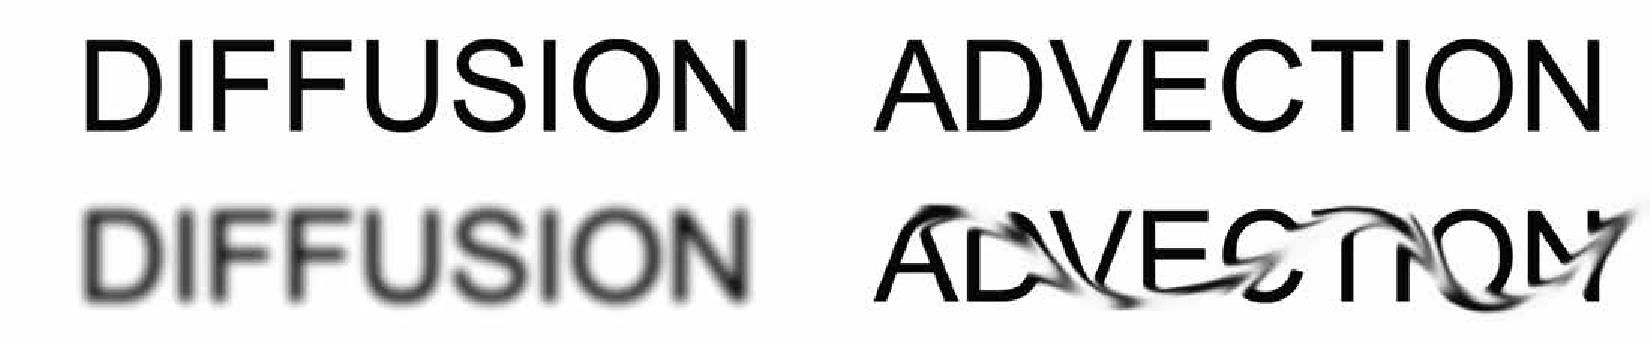
\includegraphics[width=0.95\textwidth]{06_fld/figures/fig_diffusion_vs_advection.pdf}
\caption{Illustration of diffusive (left) and advective (right) transport of particles. With diffusion, particles spread locally depending on the gradient of the particle distribution, which for flux-limited diffusion is the zero moment, the fluence. Advection is the movement of particles along a directed force field. For flux-limited diffusion, this force field is defined by the first moment, the flux vector.}
\label{fig:fld_vef_advection_diffusion}
\end{figure}


Classical diffusion assumed an isotropic distribution of radiance for the second moment, while pure streaming transport assumed a delta distribution. The Variable Eddington Factor theory assumes a radiance distribution, which is rotationally symmetric around a dominant vector $\vec{n}$. This assumption allows to derive a form for $T$, which represents isotropic distribution as well as a pure delta distribution and those forms inbetween, which are rotationally symmetric around a dominant direction $\vec{x}$.
\begin{figure}[h]
\centering
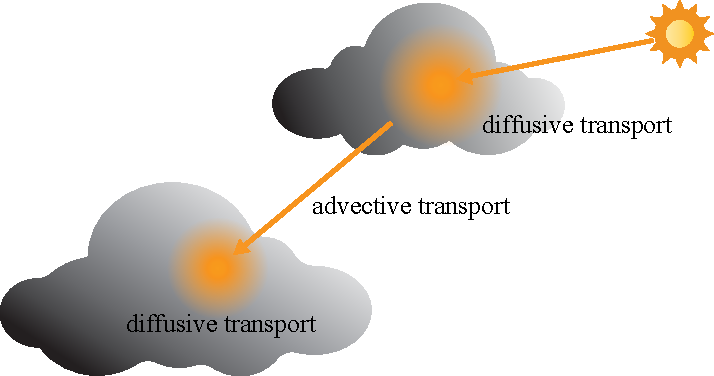
\includegraphics[width=0.55\textwidth]{06_fld/figures/fig_transport_regimes_scene.pdf}
%\missingfigure{show image with isotropic distribution, streaming limit distribution and inbetween forms}
\caption{Radiative transfer in typical scenes contains a mix of transport regimes as shown in this figure. Diffuse transport in dense media with high absorption and advective transport in thin media. The idea behind the Variable Eddington Factor is to express radiative transfer as a mix between those two extreme transport modes.}
\label{fig:fld_vef_advection_diffusion2}
\end{figure}

The Variable Eddington Factor form of $T$ is derived by considering a principal direction of transport, given by the vector $\vec{n}$ of unit length. An important assumption is that the radiance distribution will be radially symmetric around this direction. This means, that the value of $\hat{L}$ will be invariant to a rotation about axis $\vec{n}$. It follows, that its first and second moment $\hat{L}_1$ and $\hat{L}_2$ will also be invariant to rotation about $\vec{n}$. If one approximates $\hat{L}_2$ using the Eddington tensor $T$ with $\hat{L}_2\approx T\phi$, it can be concluded that $\vec{n}$ will be an eigenvector of $T$ with eigenvalue $\chi$:
\begin{align*}
T\vec{n} = \chi\vec{n}
\end{align*}
%\TD{explain/give reference why eigenvectors need to sum up to one}
The plane perpendicular to $\vec{n}$ is an eigenspace of $T$. By requiring that all eigenvalues sum up to one, the eigenvalues of the two eigenvectors spanning that plane by distributing the remaining eigenvalue $1-\chi$ evenly between both is expressed as:
\begin{align}
\frac{1}{2}\left(1-\chi\right)\mathbf{I}
\label{eq:iso_var_T_isoterm}
\end{align}
From the free streaming limit case (section~\ref{sec:fld_streaming_limit_approximation}), it is known that $\chi=1$, when the radiance distribution becomes a delta distribution (equation~\ref{eq:zero_moment_Lhat} and~\ref{eq:first_moment_Lhat}). In that case, the eigenvalues associated with the eigenvectors perpendicular to $\vec{n}$ become zero and the term above vanishes.

Tensor diagonalization allows to explicitly add the eigenvector $\vec{n}$ by adding the matrix $\vec{n}_i\vec{n}_j$ (with $\vec{n}$ being of unit length). The scaling of its coefficients is found by considering that the term in equation~\ref{eq:iso_var_T_isoterm} introduces three eigenvectors. The sum of their eigenvalues will be $3/2(1-\chi)$. Since eigenvalues of the final tensor $T$ need to add up to one, the eigenvalue associated with the matrix $\vec{n}_i\vec{n}_j$ will be $\left(1- \frac{3}{2}\left(1 - \chi\right)\right)$. This results in the following form for $T$:
\begin{align}
T &= \frac{1}{2}\left(1-\chi\right)\mathbf{I} + \left(1- \frac{3}{2}\left(1 - \chi\right)\right) \vec{n}\otimes\vec{n}
\nonumber
\\
&= \frac{1}{2}\left(1-\chi\right)\mathbf{I} + \frac{1}{2}\left(3\chi-1\right) \vec{n}\otimes\vec{n}
\label{eq:iso_var_T}
\end{align}
This form of $T$ is called the Variable Eddington Tensor (VET). It can be understood as an \emph{interpolation} between an isotropic distribution tensor ($1/3\mathbf{I}$) and a delta distribution tensor ($\vec{n}_i\vec{n}_j$). The variable $1/3 \le \chi \le 1$ is the interpolation variable and is called the Eddington factor (VEF). Theories, which respect this structure of the Eddington tensor are referred to as theories under the variable Eddington factor formalism (VEF-formalism).

If $\chi=1/3$, then equation~\ref{eq:iso_var_T} will result in the isotropic distribution tensor, which is the base assumption for classical diffusion:
\begin{align}
\frac{1}{2}\frac{2}{3}\mathbf{I} + \frac{1}{2}\left(\frac{3}{3}-1\right) \vec{n}\otimes\vec{n}
=\frac{1}{3}\mathbf{I} + 0\vec{n}\otimes\vec{n} = \frac{1}{3}\mathbf{I}
\end{align}
For $\chi=1$, equation~\ref{eq:iso_var_T} produces the Eddington tensor, which was derived for the pure streaming limit distribution, where all light comes from a singular direction:
\begin{align}
\frac{1}{2}0\mathbf{I} + \vec{n}\otimes\vec{n}
= \vec{n}\otimes\vec{n}
\end{align}
The Eddington factor $\chi$ can also be interpreted as a measure of anisotropy of the radiance distribution $\widehat{L}$ with respect to direction $\vec{n}$. It can be expressed in terms of the radiance distribution by the squared mean cosine (given by Levermore~\cite{Levermore84}):
\begin{align}
\chi &= \int_{S^2}{ \left(\omega\cdot\vec{n}\right)^2\hat{L}\left(\vec{x}, \omega\right)\ud\omega}
\label{eq:iso_var_chi}
\end{align}
With the variable Eddington factor approach, only a function for the interpolation variable $\chi$ (the actual Eddington factor) needs to be identified. This function should have $1/3$ and $1$ as its limits. With such an interpolation function, the limit transport cases (diffusion and free streaming) will be a subset of any theory, which adheres to the variable Eddington factor concept.

The Eddington factor framework, sets up the Eddington factor and the limits of its parameterization, $\chi$. The specific expression for this factor is not defined and it is clear that there are many options for the function $\chi$, which respect the given function limits. This is why there is such a rich variety of theories in other domains, which all propose their own version of that interpolation function. Some of them are ad-hoc schemes (Bowers et al.~\cite{Bowers82}, Kershaw~\cite{Kershaw76} and Larsen et al.~\cite{Larsen74}), which are derived from heuristics, while others have a clear connection to transport theory (Levermore at al.~\cite{Levermore81}) or are derived from entropy theory (Minerbo~\cite{Minerbo78}).

The general strategy for all these different variable Eddington factor theories is:
\begin{enumerate}
\item Find a model or theory, from which a certain radially symmetric form of the radiance distribution $\hat{L}$ about the normalized flux-vector$\vec{E}/\phi$ can be found or justified.
\item Then derive an expression for $\chi(\vec{E}/\phi)$ from the model for $\hat{L}$, which can be used to construct $T$. Further assumptions are applied, to be able to express $\vec{E}$ in terms of $\nabla\phi$. This is required in order to not have $T$ depend on the flux-vector directly as it still needs to be possible to resolve equation~\ref{eq:me_first_resolved_E} for the flux-vector.
\end{enumerate}

In this thesis, results for different theories have been presented and implemented, but only flux-limited diffusion from Levermore et. al~\cite{Levermore81} was discussed, since it is the most popular and also has the strongest connection to transport theory. Discussing all other theories is beyond the scope of this thesis and also not really necessary, as it is shown in section~\ref{sec:fld_results} that the particular choice of theory is not of significant importance for applications in computer graphics.






\section{Eddington Factors and Flux-limiters}
\label{sec:fld_vef_factors}

\section{Non-Linear Gauss-Seidel Solver with Successive Overrelaxation}
\label{sec:fld_solver}

\section{Results}
\label{sec:fld_results}

\TD{mention publication}
\TD{mention application in elementacular}